
Utilizzando  GWT-RPC  tutte  le  chiamate  effettuate  dalla  pagina  HTML  al  server 
sono  asincrone.
Questo  significa  che  le  chiamate  non  bloccano  il  client  mentre attende   una 
risposta   dal   server,   ma   viene  eseguito   il   codice   immediatamente 
successivo.

\begin{figure}[!htb]
\centering%
\includegraphics[scale=0.5]{AnatomySVG.png}%
\caption{GWT-RPC }\label{fig:GWT-RPC}%
\end{figure}

\FloatBarrier
Utilizzando GWT-RPC, i nostri oggetti del modello vengono automaticamente serializzati quando vengono utilizzati come parametri per una chiamata RPC. Le uniche restrizioni sono date dall’obbligatorietà di implementare 
\subsection{Comunicazione con server}
l’interfaccia Serializable e dalla presenza di un costruttore senza argomenti. 

Il primo passo per l’attuazione del servizio RPC è quello di dichiarare l’interfaccia di servizio che estenda l’interfaccia RemoteService ed elenchi tutti i metodi RPC.
Successivamente definire una classe per implementare il codice server-side che estenda la classe RemoteServiceServlet ed implementi l’interfaccia creata precedentemente. 
Ora non rimane che implementare la versione asincrona dell'interfaccia per l’applicazione client poiché ogni metodo chiamato deve essere asincrono.

\begin{figure}[!htb]
\centering%
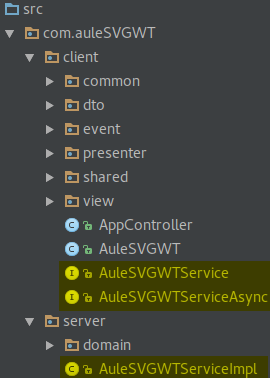
\includegraphics[scale=0.55]{rpcPack.png}%
\caption{Classi utilizzate per il servizio RPC. }\label{fig:RPCPack}%
\end{figure}